\documentclass{report}
\usepackage[utf8]{inputenc}
\usepackage{minted}
\usepackage[margin=0.7in]{geometry}

\usepackage{biblatex} %Imports biblatex package
\usepackage[toc,page]{appendix}
\usepackage{siunitx}
\usepackage{mathrsfs,mismath,amsfonts,amssymb,amsmath,mathabx, braket,diagbox,hhline}
\usepackage{graphicx}
\usepackage{epstopdf}

\addbibresource{library.bib} %Import the bibliography file
\title{Continuous Error Correction in Quantum Dot Qubits}
\author{Stasiu Wolanski, Jesus College}
\date{2022 - 2023}

\begin{document}

\maketitle

\begin{abstract}
    Woop!
\end{abstract}

\tableofcontents

\section{Introduction}
\chapter{Background}

\section{Quantum error correction}
\subsection{Quantum computing}
\subsection{Error correction}
\subsection{Continuous error correction}


\section{Quantum Dot Qubits}
\subsection{Semiconductor Heterostructures}
\subsubsection{The Hubbard Model} \label{sec:hubbard_model}

\chapter{Theory}

\section{Rapidly repeated error correction schemes} \label{sec:repeat_analysis}

\section{Truly continuous error correction in quantum dot systems} \label{sec:truly_continuous_theory}
\begin{figure}[h]
    \centering
    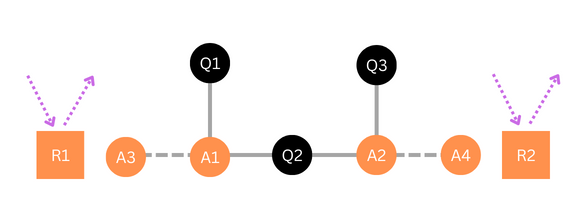
\includegraphics[scale = 1]{Figures/7qubitlayout.png}
    \caption{Schematic of the layout of qubits for the continuous error correction scheme. Q1, Q2 and Q3 comprise a single logical qubit. A1 to A4 are ancilla qubits used to detect bit flip errors in the logical qubits. Q1 and Q2 are continuously weakly coupled to A1 through a tunnel barrier, and likewise Q2 and Q3 to A2. R1 and R2 are resonators, which are additional quantum dots held at a higher electron occupancy than the qubits. These are probed using RF signals, and their coupling to the charge on the ancillas then allows the singlet/triplet state of the ancillas, as in \cite{Oakes2022}.}
    \label{fig:7qubitlayout}
\end{figure}
\subsection{Scheme summary}

In this section a proposal for truly continuous error correction is developed. I thank Chris Long, Dr Mertig, Giovanni Oakes and my supervisor Dr Arvidsson-Shukur for contributing variously to the development of the ideas presented here. Recent developments in the field of RF reflectometry measurements enable the measurement of the singlet/triplet state of two adjacent qubits coupled via a tunnel barrier, by monitoring the rf reflection characteristics of a neighbouring electron reservior \cite{Oakes2022}. The codespace qubits are to be coupled pairwise to two ancilliary qubits whose function is to perform parity measurements, in such a way that any deviation from the codespace will result in a change of state of one or both of the ancilla qubits, depending on the error syndrome. The rate at which the error propogates to the ancilla qubit(s) is in the tens of nanoseconds, a faster timescale than either gate times (hundreds of nanoseconds) or readout (the state of the art \cite{Oakes2022} achives 6\unit{\micro\second}). 

This scheme is potentially more efficient than a repeated error correction scheme like those analysed in section \ref{sec:repeat_analysis}. One reason for this is that the `dead time' after an error has occurred during which the system is vulnerable to a second error is limited by the time for the ancilla to be reset, which is also on the order of microseconds (e.g. see \cite{Nakajima2019}). A second, more significant advantage is that the scheme does not require any quantum gates to be performed for the purposes of error sydrome detection, as such detection happens continuously and simultaneously with circuit gates. This reduces circuit complexity, and avoids the error accumulation associated with performing the syndrome measurements. 

TODO flesh this out.



The proposed qubit layout is given in figure \ref{fig:7qubitlayout}. The nature of the circuit requires a 2D array of quantum dot structures, of which there is not yet any published experimental demonstration, but a proposed architecture was proposed in \cite{Tadokoro2021_2}. In the scheme, the logical qubit is encoded in the \textit{odd parity subspace} of three qubits Q1, Q2, and Q3. There are two pairs of ancilla qubits: A1, A3, and A2, A4. Each of these is initially prepared in the $T_0$ triplet state. As shown in the figure, each pair of qubits Q1 and Q2, Q2 and Q3, is weakly coupled to one ancilla qubit through a voltage-controlled tunnel barrier. If the couplings are sufficiently well-tuned, the ancilla qubits will remain as triplets and no tunneling will occurr. When a bit-flip error occurrs on one of Q1, Q2 or Q3, this will cause one or both (depending on the error syndrome) of the ancilla pairs to rotate into a singlet state. This allows (subject to complexities discussed in section \ref{sec:tunneling_question}) tunneling between the electrons in the affected pair, which is registered as a change in dispersive response of the nearby resonator. Thus the error syndrome is immediately detected as a signal in the continuously monitored reflectometry circuit.

\subsection{Theoretical treatment of scheme with second order perturbation theory}

Suppose the system is initally in an arbitrary codespace state, with each of the ancilla pairs starting in triplet states:
\begin{equation*}
    \ket{\psi(t = 0)} = (\alpha\ket{\uparrow_{Q1}\downarrow_{Q2}\uparrow_{Q3}} + \beta\ket{\downarrow_{Q1}\uparrow_{Q2}\downarrow_{Q3}})(\ket{\uparrow_{A1}\downarrow_{A3}} + \ket{\downarrow_{A1}\uparrow_{A3}})(\ket{\uparrow_{A2}\downarrow_{A4}} + \ket{\downarrow_{A2}\uparrow_{A4}}) / 2
\end{equation*}
First consider the case where no coupling is applied between the qubits. If we can engineer our system so that $\delta_{1,3}^z = E_{A1}^z - E_{A3}^z \ll 1/T_1$, and similarly $\delta_{2,4}^z \ll 1/T_1$ (with $T_1$ the timescale of bit flip errors), then the energy difference between the two branches of each qubit singlet is sufficiently small that rate at which the triplets rotate into triplets, and so register a tunnelling event on the reflectometry apparatus, is long compared to the error time and so not limiting. We can see this by considering a single ancilla branch:
\begin{equation}
    \ket{\psi(t)} = \frac{1}{\sqrt{2}}(\ket{\uparrow\downarrow} + \exp(-2i\delta t)\ket{\downarrow\uparrow}) = \frac{1}{2}\ket{T_0}(1 + \exp(-2i\delta t)) + \frac{1}{2}\ket{S_0}(1 - \exp(-2i\delta t)))
\end{equation} \label{eq:triplet_to_singlet}, so that the amplitude of the singlet state goes as 
\begin{equation*}
    \left|\braket{S_0|\psi(t)}\right|^2 = \sin(\delta t)^2
\end{equation*}.

Now we apply a coupling between the following four pairs of qubits: Q1 and A1, Q2 and A1, Q2 and A2, Q3 and A2. We consider the four branches of the state in the computational basis of the ancilla qubits seperately, and apply second order perturbation theory to approximate the energy shift of each state due to the adiabatic application of a weak coupling, of strength $t$. The limits of this approximate treatment will be tested using a numerical simulation developed in chapter \ref{chap:methods}.

The standard formula for second order perturbation theory is (there is no first-order shift in energy as the perturbing terms are off-diagonal):

\begin{equation*}
    E_i^1 \approx E_i^0 + \sum_j{\frac{|\braket{\psi_i|V|\psi_j}|^2}{E_i^0 - E_j^0}}
\end{equation*} where $E_i^0$ and $E_i^1$ are the unperturbed and perturbed energies of state $i$, and $H_0$ and $V$ are the basic and perturbative hamiltonians. If we set $V$ to the hopping term in the hubbard model, then we obtain, for example,
\begin{align*}
    E_{\uparrow\downarrow\uparrow,\uparrow\downarrow,\uparrow\downarrow}^1 - E_{\uparrow\downarrow\uparrow,\uparrow\downarrow,\uparrow\downarrow}^0 &= 
    -\frac{t^2}{E_{\uparrow\updownarrow \uparrow,\varnothing\downarrow,\uparrow\downarrow}^0 - E_{\uparrow\downarrow\uparrow,\uparrow\downarrow,\uparrow\downarrow}^0}
    -\frac{t^2}{E_{\uparrow\varnothing \uparrow,\updownarrow\downarrow,\uparrow\downarrow}^0 - E_{\uparrow\downarrow\uparrow,\uparrow\downarrow,\uparrow\downarrow}^0}
    -\frac{t^2}{E_{\uparrow\updownarrow \uparrow,\uparrow\downarrow,\varnothing\downarrow}^0 - E_{\uparrow\downarrow\uparrow,\uparrow\downarrow,\uparrow\downarrow}^0}
    -\frac{t^2}{E_{\uparrow\varnothing \uparrow,\uparrow\downarrow,\updownarrow\downarrow}^0 - E_{\uparrow\downarrow\uparrow,\uparrow\downarrow,\uparrow\downarrow}^0}\\
    &= -t^2\left(\frac{1}{\Delta_1} + \frac{1}{\Delta_2} + \frac{1}{\Delta_3}+ \frac{1}{\Delta_4}\right)
\end{align*} with
\begin{align*}
    \Delta_1 &= U_{Q2} + \mu_{Q2} - \mu_{A1} + \E_{Q2}^z - \E_{A1}^z \\
    \Delta_2 &= U_{A1} + \mu_{A1} - \mu_{Q2} + \E_{Q2}^z - \E_{A1}^z \\
    \Delta_3 &= U_{Q2} + \mu_{Q2} - \mu_{A2} + \E_{Q2}^z - \E_{A2}^z \\
    \Delta_4 &= U_{A2} + \mu_{A2} - \mu_{Q2} + \E_{Q2}^z - \E_{A2}^z \\
\end{align*}, where the terms describe parameters of the Hubbard model described in section \ref{sec:hubbard_model}.

We note that $U_i \gg \Delta \mu_i, E^z_i$, and that the magnitude of $U_i$ (order of a few \unit{\milli\electronvolt}) varies little from site to site , so that we may define $\Lambda_t = 2t^2/\braket{U_i}$. Then we have 
\begin{equation*}
    E_{\mathrm{C}\uparrow\downarrow,\uparrow\downarrow}^1 - E_{\mathrm{C}\uparrow\downarrow,\uparrow\downarrow}^0  = \Delta E_{\mathrm{C}\uparrow\downarrow,\uparrow\downarrow} \approx
    \Delta E_{\mathrm{C}\uparrow\downarrow,\downarrow\uparrow} \approx
    \Delta E_{\mathrm{C}\downarrow\uparrow,\uparrow\downarrow} \approx
    \Delta E_{\mathrm{C}\downarrow\uparrow,\downarrow\uparrow} \approx -2\Lambda_t
\end{equation*}, where we note the shift in energy is the same, within the above approximations, for both of the codespace branches, $\ket{\uparrow\downarrow\uparrow}$ and $\ket{\downarrow\uparrow\downarrow}$, and denote the energies of both branches by the subscript C. All branches of the ancilla state will therefore accure phase at the same rate as long as the state code qubits remains within the codespace.

\newcommand{\dlam}[2]{\diagbox{$#1\Lambda_t$}{$#2\Lambda_t$}}
\begin{table}
    \centering
\begin{tabular}{|c|c||c|c|c|c|}
\hline
\multicolumn{2}{|c||}{Computational branch} & \multicolumn{4}{c|}{Ancilla branch} \\
\hline
 Subspace & branch & $\uparrow\downarrow\uparrow\downarrow$ & $\uparrow\downarrow\downarrow\uparrow$ & $\downarrow\uparrow\uparrow\downarrow$ & $\downarrow\uparrow\downarrow\uparrow$ \\
 \hhline{|=|=||=|=|=|=|}

Codespace & \diagbox{$\uparrow\downarrow\uparrow$}{$\downarrow\uparrow\downarrow$} & $2\Lambda_t$ & $2\Lambda_t$ & $2\Lambda_t$ & $2\Lambda_t$\\
\hline
E1 & \diagbox{$\downarrow\downarrow\uparrow$}{$\uparrow\uparrow\downarrow$} & \dlam{3}{1} & \dlam{3}{1} & \dlam{1}{3} & \dlam{1}{3}\\
\hline
E2 &\diagbox{$\uparrow\uparrow\uparrow$}{$\downarrow\downarrow\downarrow$} & \diagbox{$0$}{$4\Lambda_t$} & $2\Lambda_t$ & $2\Lambda_t$ & \diagbox{$4\Lambda_t$}{$0$}\\
\hline
E3 & \diagbox{$\uparrow\downarrow\downarrow$}{$\downarrow\uparrow\uparrow$} & \dlam{3}{1} & \dlam{1}{3} & \dlam{3}{1} & \dlam{1}{3}\\
\hline
\end{tabular}
\caption{Table of the (negative) energy shifts due to coupling of each ancilla branch, of each computational branch, of each subspace.}\label{table:shifts}
\end{table}


When a bit-flip error occurs, the state will aquire a component in one of the error subspaces, denoted E1, E2 and E3 depending on which qubit has flipped. Applying the above analysis, we calculate the energy shifts of each of the ancilla branches of each computational branch in each codespace. These are given in table \ref{table:shifts}. These shifts result in the A1, A3, or A2, A4 ancilla pairs rotating from triplets to singlets, or both, depending on the error subspace. To see this, consider the E1 error subspace, into which the state moves when the Q1 qubit experiences a bit-flip error. If both ancilla pairs are in triplet states at the point when the system transitions into the E1 subspace from the codespace, the state undergoes the following evolution \footnote{We assume that the resultant state is approximately a stationary state of the perturbed hamiltonian.}:

\begin{align*}
    \ket{\psi(t)} = &\alpha\ket{\downarrow\downarrow\uparrow}(
        e^{-3 i \Lambda_t t }\ket{\uparrow\downarrow\uparrow\downarrow} 
    + e^{-3 i \Lambda_t t }\ket{\uparrow\downarrow\downarrow\uparrow}
    + e^{-i \Lambda_t t }\ket{\downarrow\uparrow\uparrow\downarrow}
    + e^{-i \Lambda_t t }\ket{\downarrow\uparrow\downarrow\uparrow})/2 \\
    + e^{-i\delta_{Q1,Q3} t} &\beta\ket{\uparrow\uparrow\downarrow}(
        e^{- i \Lambda_t t }\ket{\uparrow\downarrow\uparrow\downarrow} 
    + e^{- i \Lambda_t t }\ket{\uparrow\downarrow\downarrow\uparrow}
    + e^{-3i \Lambda_t t }\ket{\downarrow\uparrow\uparrow\downarrow}
    + e^{-3i \Lambda_t t }\ket{\downarrow\uparrow\downarrow\uparrow})/2 \\
    &\approx e^{-3 i \Lambda_t t}\alpha\ket{\downarrow\downarrow\uparrow}
    (\ket{\uparrow\downarrow} + e^{2 i \Lambda_t t }\ket{\downarrow\uparrow})
    (\ket{\uparrow\downarrow} + \ket{\downarrow\uparrow})/2 \\
    &+ e^{- i \Lambda_t t}\beta\ket{\uparrow\uparrow\downarrow}
    (\ket{\uparrow\downarrow} + e^{-2 i \Lambda_t t }\ket{\downarrow\uparrow})
    (\ket{\uparrow\downarrow} + \ket{\downarrow\uparrow})/2
\end{align*}, where the $\delta_{Q1, Q3}$ phase term accounts for the difference in energy between the two branches, which is small compared to $\Lambda_t$, and irrelevant to our conclusion, so we ignore it. By comparison with equation \ref{eq:triplet_to_singlet}, we see that the A1,A3 ancilla pair in both branches will rotate into a triplet state with a characteristic timescale $1/\Lambda_t$. The same analysis yields for E2 error subspace:
\begin{align*}
    \ket{\psi(t)} \approx &\alpha\ket{\downarrow\downarrow\uparrow}
    (\ket{\uparrow\downarrow} + e^{ -2 i \Lambda_t t }\ket{\downarrow\uparrow})
    (\ket{\uparrow\downarrow} + e^{ -2 i \Lambda_t t }\ket{\downarrow\uparrow})/2 \\
    + e^{-4 i \Lambda_t t} &\beta\ket{\downarrow\downarrow\uparrow}
    (\ket{\uparrow\downarrow} + e^{ 2 i \Lambda_t t }\ket{\downarrow\uparrow})
    (\ket{\uparrow\downarrow} + e^{ 2 i \Lambda_t t }\ket{\downarrow\uparrow})/2
\end{align*}, so that both pairs of ancillas rotate into singlets. The E3 case is identical to the E1 case with the appropriate qubits exchanged, and leads to only the A2, A4 qubit pair rotating into a singlet.

\subsection{Further questions related to tunnelling physics} \label{sec:tunneling_question}

Much work has been done optimising the implementation and and examining the classical physics of reflectometry as a tool for quantum measurement. For a review see, e.g. \cite{Vigneau2023}, especially section VIII. During the project the author has not had time to study the physics behind this technique in detail. It appears, however, that present analyses treat the system semi-classically in assuming that an electron tunnels, or does not, within the measurement period (i.e. the period of time that the tunneling barrier between the pair of qubits is lowered). They then seek to maximise the fidelity with which this charge-shifting event, or lack thereof, is detected. This tunneling event is interpreted as a projective measurement of the singlet/triplet system at the point of measurement, with probabilities of either state given by Born's rule. In the present case this is an insufficient analysis: at any given time, there is necessarily some finite component of the electron pair state that is a singlet, and we need to establish a rate at which tunnelling occurs as a function of the amplitude of this component. A full treatment of this problem probably needs to be formulated in terms of quantum master equations and the theory of quantum decoherence \cite{Wiseman1996}.

Time has not permitted me to look into this issue, so at the suggestion of my supervisor I will make the simplifying assumption that any ancilla pair that aquires more than a 10\% square-amplitude of singlet immediately tunnels and is hence registered by the dispersive readout device with empirically determined fidelity.

\chapter{Methods} \label{chap:methods}

\section{Simulating the hubbard model}
This section will discuss the methodology used to perform simulations of scheme described in section \ref{sec:truly_continuous_theory} on a hubbard model of a multiple quantum dot system. The treatment of the error correction scheme described in section \ref{sec:truly_continuous_theory} is necessarily highly approximate due to the complexity of the high-dimensional hilbert space involved (for 7 electrons on 7 sites, the occupation basis is of dimension 3432) and the large number of parameters of the Hubbard model, so makes multiple simplifying assumptions, chiefly the application of second-order perturbation theory and ignoring the site-to-site variance in certain model parameters. It is therefore valuable to simulate the Hubbard model numerically to test the validity of these assumptions in various parameter regimes.

My supervisor Dr. Arvidsson-Shukur have developed a code (yet unpublished), \texttt{DotHamiltoniser}, designed to generate Hubbard hamiltonians in an occupation basis given a set of physical parameters ($E_i^z, U_i$, etc.), as well as to perform low-dimensional time-evolution simulations. This was very helpful at the start of my project to visualise the energy levels of the system and their dependence on coupling, but was not designed for higher dimensional time evolution, and could not be used for this purpose due to performance limitations.

I therefore designed a Hamiltonian simulation code, inspired by the work of Dr Arvidsson-Shuker et al., with the ability to handle higher dimensional systems. The system has three main components: 
\begin{enumerate}
    \item A python extension, \texttt{FastHamiltoniser}, written in C, C++ and CUDA, which provides highly performant specialised sparse matrix operations for use in Hamiltonian time evolution;
    \item \texttt{Hamiltonian}, a python class that builds a Hubbard model Hamiltonian from physical parameters; and
    \item \texttt{Evolution}, a python class which takes as input a Hamiltonian and a set of continuous time instructions to produce a time evolution of a given starting statevector.
\end{enumerate}
\subsection{Python extension: \texttt{FastHamiltoniser}}
\begin{figure}[h]
    \centering
    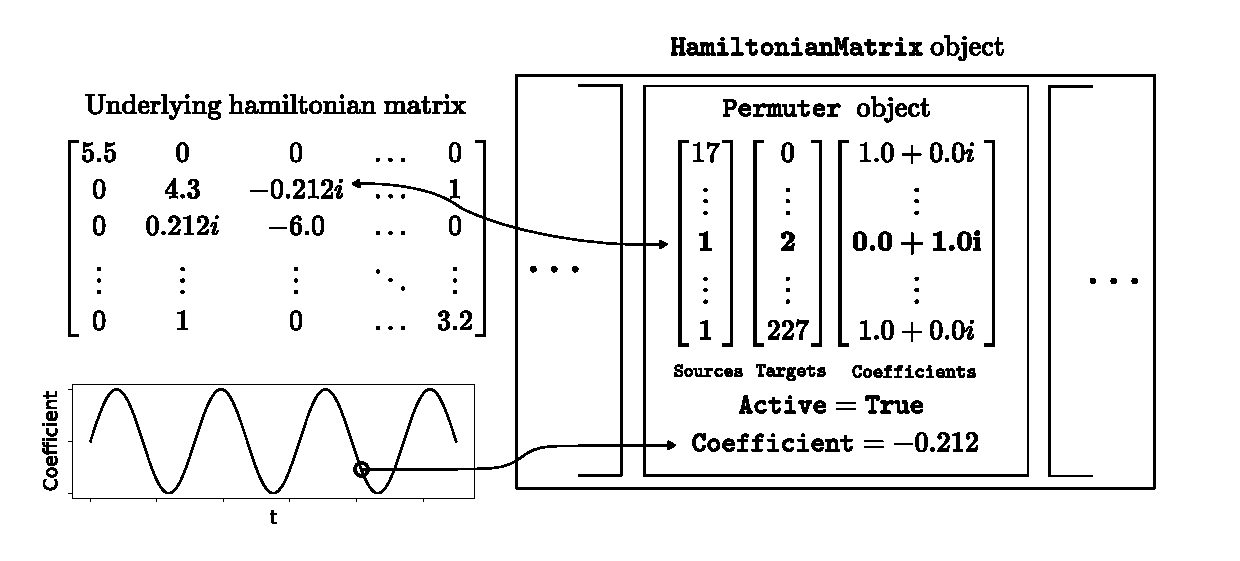
\includegraphics[scale = 0.8]{Figures/fasthamiltoniser/diagram.pdf}
    \caption{How sparse Hamiltonian matrices are represented in the custom python extension \texttt{FastHamiltoniser}. The non-zero matrix elements are grouped into objects of type \texttt{Permuter}, whose structure is calculated in advance but whose activation and multiplicative coefficients are modified efficiently as runtime.}
    \label{fig:fasthamiltoniser}
\end{figure}
\subsubsection{Structure of extension}
The purpose of the simulator is to solve the Schrödinger equation
\begin{equation} \label{eq:schrodinger}
    \dot{\psi} = -i H \psi 
\end{equation} (here expressed in natural units $\hbar = 1$) where $\psi$ is a vector in the occupation basis of a Hubbard Hamiltonian. In order to use Runge-Kutta \cite{Butcher1996} methods of integration, we need to be able to calculate this derivative efficiently at an arbitrary time and with arbitrary input. $H$ is typically very sparse, with the only off-diagonal terms given by magnetic drives and hopping couplngs, of which typically only a subset of size linear in the number of qubits are non-zero at a given time. 

To perform this calculation efficiently, I implemented the following data structure in C. A \texttt{HamiltonianMatrix} object, illustrated in figure \ref{fig:fasthamiltoniser}, contains basic data about the dimension of the array, as well as an array of pointers to objects of type \texttt{Permuter}. Each of these \texttt{Permuter} objects stores three arrays of equal length, two of integers representing source and target vector indices, and one of floats representing matrix coefficients, where each entry represents a matrix element. \texttt{Permuter}s also store a complex coefficient, which can be changed over time by writing to a single variable, and a boolean representing whether it is `on' or `off'. The internal arrays are determined in advance of the simulation by python code, and thereafter only the strength and activations of the \texttt{Permuter} objects need be modified during the simulation. For example, one such object provides all the on-diagonal elements of the matrix, and another might provide all the off-diagonal elements associated with a particular J-coupling between two qubits.

The calculation \ref{eq:schrodinger} can then be performed by iterating over the active permuters and building up the derivative vector according to the permutation and coefficient arrays. 
\subsubsection{Interaction picture calculation}
A further requirement that favoured the development of a custom C backend was the ability to perform simulations in the interaction picture. Performing simulations in the interaction picture is necessary due to the large differences in energy between eigenstates, for example due to the $U_i$ on-site repulsion in some states. With any choice of reference energy in a static basis, there are always states whose phase rotate much faster than the timescale of the evolutions that I wish to simulate, meaning there is no suitable step-size that captures the desired phenomena within reasonable computational time with the simulation remaining stable. Instead, we perform the following transformation to the interaction picture:
\begin{align*}
    \dot{\psi_i} &= -i\sum_j{H_{ij}\psi_j}\\
     \psi_i \rightarrow \phi_i &= e^{-i H_{ii} t} \psi_i \\
    \Rightarrow \dot{\phi} &= -i\sum_{j\ne i}{e^{- i (H_{jj} - H_{ii})t} H_{ij}\phi_j}
\end{align*}.

Since most off-diagonal terms $H_{ij}$ are zero at most points in time, this results in most states being stationary and lowering the rate of rotation of affected states to a longer timescale that can be simulated. It introduces the additional complexity, however, of introducing a time-dependence into the hamiltonian. I wrote a C function to perform the modified matrix multiplication, calculating the phase factors as required.

\subsubsection{GPU acceleration}
The calcluation to be performed is parallel in nature, and thus a candidate for GPU acceleration. I wrote the requisite kernels\footnote{This presented a lot of technical challenges as the process for incorporating CUDA C++ into python C extensions and compiling them is not documented and very technical. I made a template project with the setup to use in the future: https://github.com/Stasiu51/TemplateCudaEx} to perform the matrix multiplication in CUDA, a variant of C++ developed by Nvidia to control their graphics processing units (`GPU's) \cite{cuda}, one of which (a P620 Quadro) is installed in my laptop. On testing, the CUDA variant outperformed the CPU calculation only for systems with more than around 15 qubits, more than required and where the speed of computation is too slow for practical use anyway ($<10$ iterations per second, several orders of magnitude too slow for the simulations of the present project).

\subsection{Python class for Hubbard model construction: \texttt{Hamiltonian}}
This is a python class (and supporting code) that implements a Hubbard Hamiltonian, using \texttt{FastHamiltoniser} as a backend to store the underlying matrix. In particular it
\begin{enumerate}
    \item creates a list of basis vectors, represented as bit strings (with convenience functions for printing them in canonical notation), that span the fock basis of a system with a specified number of sites and number of electrons;
    \item defines creation and annhilation operators on these states, which it uses to
    \item construct the diagonal \texttt{Permuter} object that represents the self-energy terms due to chemical potential, coulomb repulsion, and static magnetic z-fields; and to
    \item construct the off diagonal \texttt{Permuter} objects generated by hopping terms and x and y magnetic fields. It also
    \item provides transformations to and from the interaction picture; and
    \item provides functions for creating projector and X matrices in the fock basis, which are more involved to calculate than in the computational (single electron per site) basis. 
\end{enumerate}

\subsection{Python class for time evolution of statevector: \texttt{Evolution}}

This class takes a reference to a \texttt{Hamiltonian} object, and a set\footnote{There is in fact only one such object, as they are defined in a recursive tree structure.} of objects that subclass the abstract base class \texttt{TimeStep} whose role is to provide instructions as to how to modify the parameters of the Hubbard model at given time. For example, one such object instructs the simulation to ramp a set of hopping couplings to a specified value over a given period of time, and another might oscillate the strength of the x component of the applied magnetic field at a given frequency and phase.

The \texttt{scipy} routine \texttt{solve\_ivp} is used along with the calculations of the derivative described above in a Runge-Kutta 5th order \cite{Butcher1996} integration routine to calculate the evolution of a given initial statevector. The routine is designed to estimate the errors and dynamically choose a step size for the integration. This works poorly in the present use case, as the calculated (vector-norm) error scales with the number of non-zero elements of the vector. Instead, the code allows the user to manually specify a step size, typically around $1/10$ of the smallest relevant timescale of the system, and checks the continued normalisation of the statevector as an imperfect check on the stability of the simulation.

Some demonstrations of the simulator and the results of a benchmarking exercise are shown in figure \ref{fig:benchmark}. 
\begin{figure}[h]
    \centering
    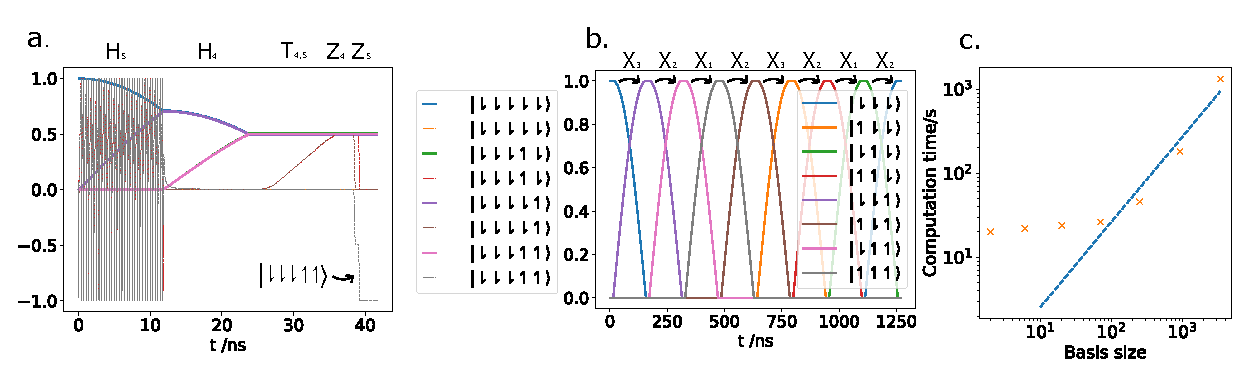
\includegraphics[scale = 0.85]{Figures/benchmark/benchmarks.pdf}
    \caption{Testing the capabilities of the simulation software. \textbf{a.} A plot of 5-qubit system showing the amplitudes (solid lines) and phases (dashed lines) of significant basis states. The plot demonstrates of a CPHASE gate acting on the last two qubits, so that the $\ket{\downarrow\downarrow\downarrow\uparrow\uparrow}$ state acquires a phase shift of $\pi$. First an X gate is applied to each of the two qubits, then a coupling between them is applied, and finally a z-rotation is applied by increasing the static field\protect\footnotemark. \textbf{b.} A sequence of X flips on a 3-qubit system. This circuit is generalised to N qubits to benchmark the simulator, with results given in \textbf{c.}. The results indicate a consistent speed of around 7.5 million statevector derivative elements calculated per second.}
    \label{fig:benchmark}
\end{figure}
\footnotetext{Applying a Z unitary rotation is not a capability typically built into such processors as it is unnecessary due to a technique called $Rz$ delaying (see, e.g. \cite{Nielsen2010} chapter 4.), but I implement it here to make the operation of the CPHASE clearer.}
\section{Truly continuous error correction prototype}
This section explains how the software described above was used to simulate the `truly continuous' error correction scheme developed in section \ref{sec:truly_continuous_theory}. In particular, we want to explore suitable physical parameters, such that when we initialise the system in an initial codespace state, and adiabatically turn on a weak coupling between the relevant qubits
\begin{itemize}
    \item the ancilla pairs remain in triplet states as long as the system remains in the codespace, for at least a time scale longer longer than ; and
    \item when a bit-flip error is artificially introduced, one or both of the ancilla pairs rotates into a singlet, as appropriate to the error syndrome.
\end{itemize}

\subsubsection{Physical parameters}
It is useful to survey the orders of magnitude of the various physical paramters of the experiment based on theoretical and experimental work to date. These can be found in table \ref{table:parameters}. As this is an exploratory piece of thoeretical work, I will take these as fairly liberal bounds.

\begin{table}
    \centering
\begin{tabular}{|c|c|c|c|}
    \hline
    Parameter & Symbol & Range & Example Reference\\
    \hline
    On-site coulomb repulsion & $U_i$ & $\sim 1\mathrm{Ry} \sim$ 1-10 \unit{\milli\electronvolt} & \cite{Shim2022}\\
    \hline 
    Static magnetic ($z$) field & $B_i^z$ & 1 - 10 \unit{\tesla} & \cite{Jock2018} \\
    \hline
    Variation in electron g factor & $\delta B_i^z$ &0.01 - 0.1 \unit{\mega\hertz} &\cite{Hwang2017} \\
    \hline
    Hopping coupling strength & $t_{ij}$ &$0.001 - 0.01$ \unit{\milli\electronvolt} & \cite{Veldhorst2015} \\
    \hline
    Phase flip coherence time &$ T_2^*$ & up to $10^3$\unit{\nano\second} in Si, $10^5$\unit{\nano\second} in $^{28}$Si & \cite{Loss2022}\\
    \hline
    Bit flip coherence/relaxation time &$T_1$&up to $10^6$\unit{\nano\second} in normal Si& \cite{Loss2022}\\
    \hline

\end{tabular}
\caption{Table of the (negative) energy shifts due to coupling of each ancilla branch, of each computational branch, of each subspace.}\label{table:parameters}
\end{table}

\subsection{Hubbard Hamiltonian setup} \label{sec:reduced_basis_approx}
The software enables us to set up a qubit basis that explicitly models the qubit layout shown in \ref{fig:7qubitlayout}, with three code qubits and two pairs of ancilla qubits. This seven-qubit system has a fock basis of dimension 3432, which is just about feasible to simulate using the software I developed (simulations of sufficiently small time step take several minutes each, and there are memory limitations in storing the results). However, this can be sped up by noting that in the circuit to be simulated, the second of each pair of ancillas, A3 and A4, do not experience any coupling, so the hamiltonian is always diagonal in these dimensions. Furthermore, the ancilla part of all states that are non-zero in the simulation are constructed out of the $\ket{\uparrow\downarrow}$ and $\ket{\downarrow\uparrow}$ states with respect to these pairs of qubits, as well as non-computational states. Therefore, we may reduce our basis if we make an appropriate modification to the Hamiltonian:
\begin{align*}
    \ket{\dots \uparrow\downarrow\uparrow\downarrow} &\rightarrow \ket{\dots \uparrow\uparrow} &
    \ket{\dots \uparrow\downarrow\downarrow\uparrow} &\rightarrow \ket{\dots \uparrow\downarrow}\\
    \ket{\dots \downarrow\uparrow\uparrow\downarrow} &\rightarrow \ket{\dots \downarrow\uparrow} &
    \ket{\dots \downarrow\uparrow\downarrow\uparrow} &\rightarrow \ket{\dots \downarrow\downarrow}\\
    E_{A1}^z &\rightarrow E_{A1}^z - E_{A3}^z & E_{A2}^z &\rightarrow E_{A2}^z - E_{A4}^z
\end{align*} this does not affect the energy levels of any of the computational states, and only affects the non-computational basis states by a quantity of order $E_i^z \ll U_i$. If we accept this approximation, we can reduce our basis size to 252, which increases the simulation speed by a factor of around $14 - 20\times$ (this is a non-linear speedup as all the simulation data now fits into memory).

Also note that most variation in spin energy from site to site come from variation in the electron G factor at different sites rather than inhomogenaities in the magnetic field \cite{Hwang2017}. It is convenient and equivalent, however, to simply include these variations into the magnetic field\footnote{Although my software does have the capability to vary the electron g-factor from site to site, it is simpler not to use it. }

\subsection{Energy shifts due to hopping coupling}

\begin{figure}[h]
    \centering
    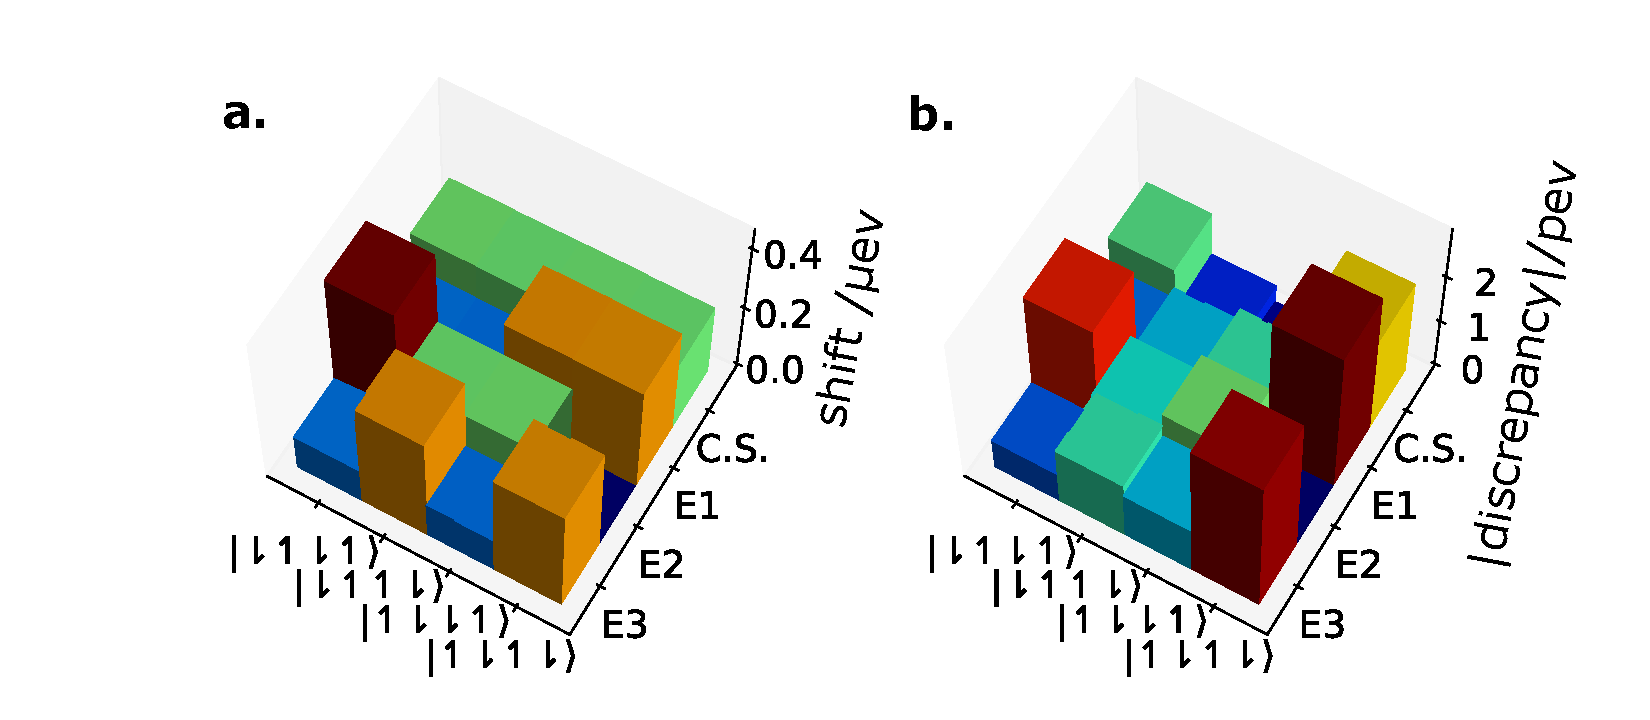
\includegraphics[scale = 0.4]{Figures/shifts.pdf}
    \caption{\textbf{a.} shows the calculation of energy shifts of the various relevant computational basis states calculated with a coupling of $0.015\unit{\milli\electronvolt}$ applied. Only one branch $\ket{\uparrow\downarrow\uparrow}$ of the computational state in each subspace is shown. This can be compared with the second order perturbation theory result calculated in table \ref{table:shifts}. The (absolute value of) the descrepancy between the simulation and the perturbation theory result is given in \textbf{b.}. Note the scale in the second plot.
    \label{fig:shifts}}
\end{figure}
It is important to know the energies of the perturbed computational states for two reasons: firstly, in order to validate the second-order perturbation theory results in section \ref{sec:truly_continuous_theory}; and secondly knowing the exact energies of these states is important if one is to use oscillating microwave signals to drive transitions between the states, to implement unitary rotations on the qubits while the coupling is active.

We find these by the following procedure: we initialise the system in the computational basis state of interest, and the hamiltonian with all couplings zero. we perform an interaction picture simulation where the couplings are ramped up to the steady state value over a time period that is sufficiently long so as to ensure adiabatic evolution of the state ($100\times\braket{U_i}^{-1}$ as this is the shortest timescale in the system). We compare this state to a list of the eigenvectors of the matrix generated by the Hamiltonian with the coupling at full strength. The eigenvector which has the maximal inner product with this state (the inner product is close to unity for the correct state, and close to zero otherwise) is the perturbed eigenvector associated with the original state in the computational basis state, and we take the associated eigenvalue as the perturbed energy.

The results for a coupling of 0.015\unit{\milli\electronvolt}, which is slightly higher than a typical coupling, and other typical experimental parameters are given in figure \ref{fig:shifts}. The simulation agrees with the perturbation theory calculation within 1\%. The agreement is closer for smaller coupling values.

\subsection{Demonstrating the error propagation}
We now want to demonstrate the process of propagation by which bit-flip errors in the code qubits Q1, Q2, Q3 result in the relevant ancilla pairs rotating into singlets, or in the reduced basis approximation decribed in \ref{sec:reduced_basis_approx}, the qubits A1 and A2 rotating from $(\ket{\uparrow} + \ket{\downarrow})/\sqrt{2}$ to $(\ket{\uparrow} - \ket{\downarrow})/\sqrt{2}$, which is equivalent.

We can acheive this by initialising the code qubits in the codespace, and then adiabatically turning on the coupling. We let this system run in steady state for enough time to establish the rate at which the singlets are introduced in the codespace. We then instantaneously apply an X unitary on one of the qubits by, and continue to let the simulation run. Afterwards, we can project the resulting time-evolved statevector data into the singlet and triplet spaces. The system prior to the bit flip is shown in figure \ref{fig:beforeflip}, and the behvaiour when a bitflip is introduced mid-way through the simulation is shown in figure \ref{fig:afterflip}.
\begin{figure}[h]
    \centering
    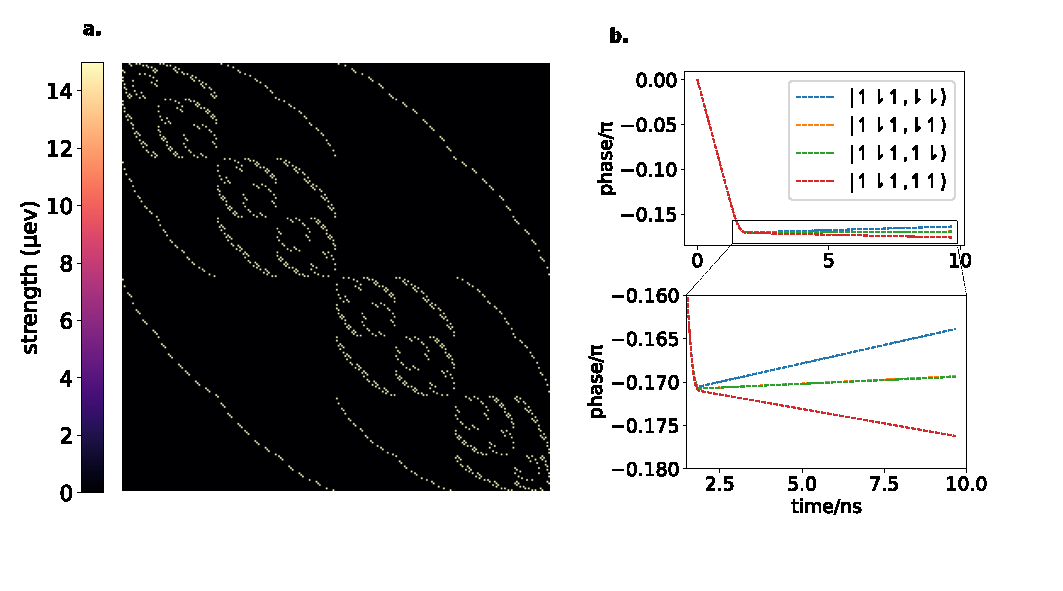
\includegraphics[scale = 1]{Figures/singlettriplet.pdf}
    \caption{The effect of applying the hopping coupling to the system still inhabilting the codespace. \textbf{a.} shows the (elementwise absolute value of the) hamiltonian matrix in the interaction picture at full strength. \textbf{b.} shows the rate of aquisition of phase of the relevant basis states. The phase initially drops when the coupling is applied, and then the states slowly drift apart from one another in phase due to the difference in electron g-factor of around 30 \unit{\mega\hertz}. At this rate, the triplet will `flip' into a singlet after around 200 \unit{\nano \second}, so this combination of parameters (coupling strength = 0.015 \unit{\milli\electronvolt}) is not be suitable for error correction. Either the coupling or the g-factor inhomogeneity needs to be reduced.
    }\label{fig:beforeflip}
\end{figure}

\begin{figure}[h]
    \centering
    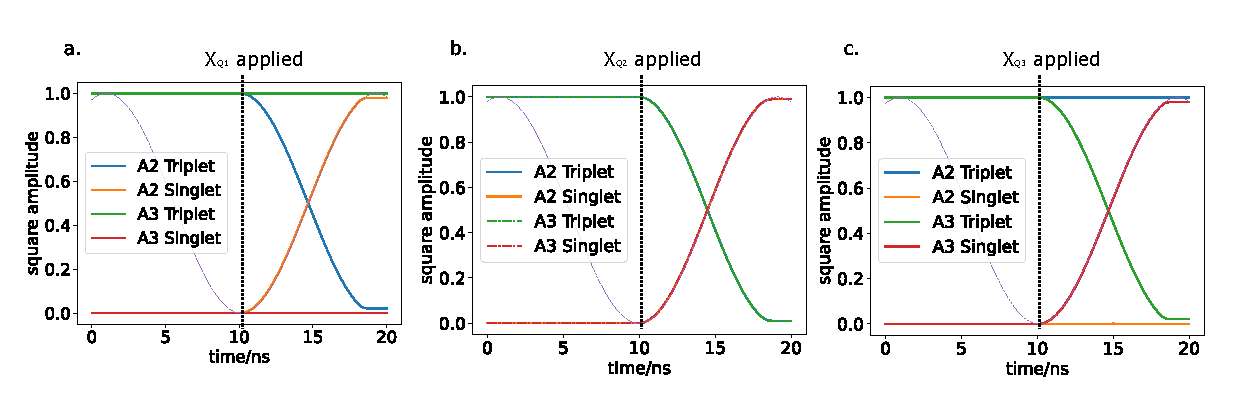
\includegraphics[scale = 0.87]{Figures/flips.pdf}
    \caption{Demonstrating the expected behaviour of the ancillas when a bit flip error is artifitially introduced on one of the code qubits: Q1 is flipped in \textbf{a.}, resulting in a rotation of the A2 ancilla; Q2 is flipped in \textbf{b.}, resulting in \textit{both} A2 and A3 rotating, and Q3 is flipped in \textbf{c.}, so that A3 rotates only. In each case, the purple dashed line shows the expected frequency of rotation derived in section \ref{sec:truly_continuous_theory}, $\Lambda_t$. Note that the period of rotation is much faster than the other typical timescales of quantum dot qubit systems.
    }\label{fig:afterflip}
\end{figure}





\chapter {Discussion}

\section{Conclusions}

\printbibliography % TODO lots of incomplete references!

\begin{appendices}
\chapter{Detecting errors in ancilla qubits.}
\chapter{Locked states}
\end{appendices}
\end{document}